\documentclass[10pt]{beamer}

\usetheme{metropolis}
\usepackage{booktabs}
\usepackage{amsmath}
\usepackage{graphicx}
\usepackage{tikz}
\usetikzlibrary{matrix,positioning}

% Python-inspired color scheme
\definecolor{pythonblue}{RGB}{55,118,171}      % Python blue
\definecolor{pythonyellow}{RGB}{255,212,59}    % Python yellow
\definecolor{pythondarkblue}{RGB}{35,75,110}   % Darker blue for contrast
\definecolor{pythonlightblue}{RGB}{106,159,181} % Lighter blue

% Apply colors to Metropolis theme
\setbeamercolor{frametitle}{bg=pythonblue, fg=white}
\setbeamercolor{progress bar}{fg=pythonyellow, bg=pythonlightblue}
\setbeamercolor{title separator}{fg=pythonyellow}
\setbeamercolor{progress bar in head/foot}{fg=pythonyellow, bg=pythonlightblue}
\setbeamercolor{progress bar in section page}{fg=pythonyellow, bg=pythonlightblue}

% Title page colors
\setbeamercolor{title}{fg=pythonblue}
\setbeamercolor{subtitle}{fg=pythondarkblue}
\setbeamercolor{author}{fg=black}
\setbeamercolor{date}{fg=pythondarkblue}

% Block colors
\setbeamercolor{block title}{bg=pythonblue, fg=white}
\setbeamercolor{block body}{bg=pythonlightblue!20, fg=black}

% Alert and example blocks
\setbeamercolor{block title alerted}{bg=pythonyellow, fg=black}
\setbeamercolor{block body alerted}{bg=pythonyellow!20, fg=black}

% Itemize/enumerate colors
\setbeamercolor{itemize item}{fg=pythonblue}
\setbeamercolor{itemize subitem}{fg=pythonblue}
\setbeamercolor{enumerate item}{fg=pythonblue}

% Standout frames (for section dividers)
\setbeamercolor{standout}{bg=pythonblue, fg=white}

\title{Why Everyone is Talking About GPUs}
\date{October 11, 2025}
\author{Dhruv Nigam}
\institute{MumPy Meetup}

\begin{document}

\maketitle

% Introduction Slide
\begin{frame}{About Me}
  \begin{itemize}
    \item Lead MLE at Dream 11
    \item Built massive ML systems at Philips, CLSA, Protium and Dream11
    \item Spent a lot of time and money(not mine) on GPUs
  \end{itemize}
  
\end{frame}

% Slide 1: NVIDIA Stock - Conversation Starter
\begin{frame}[plain]
  \begin{center}
    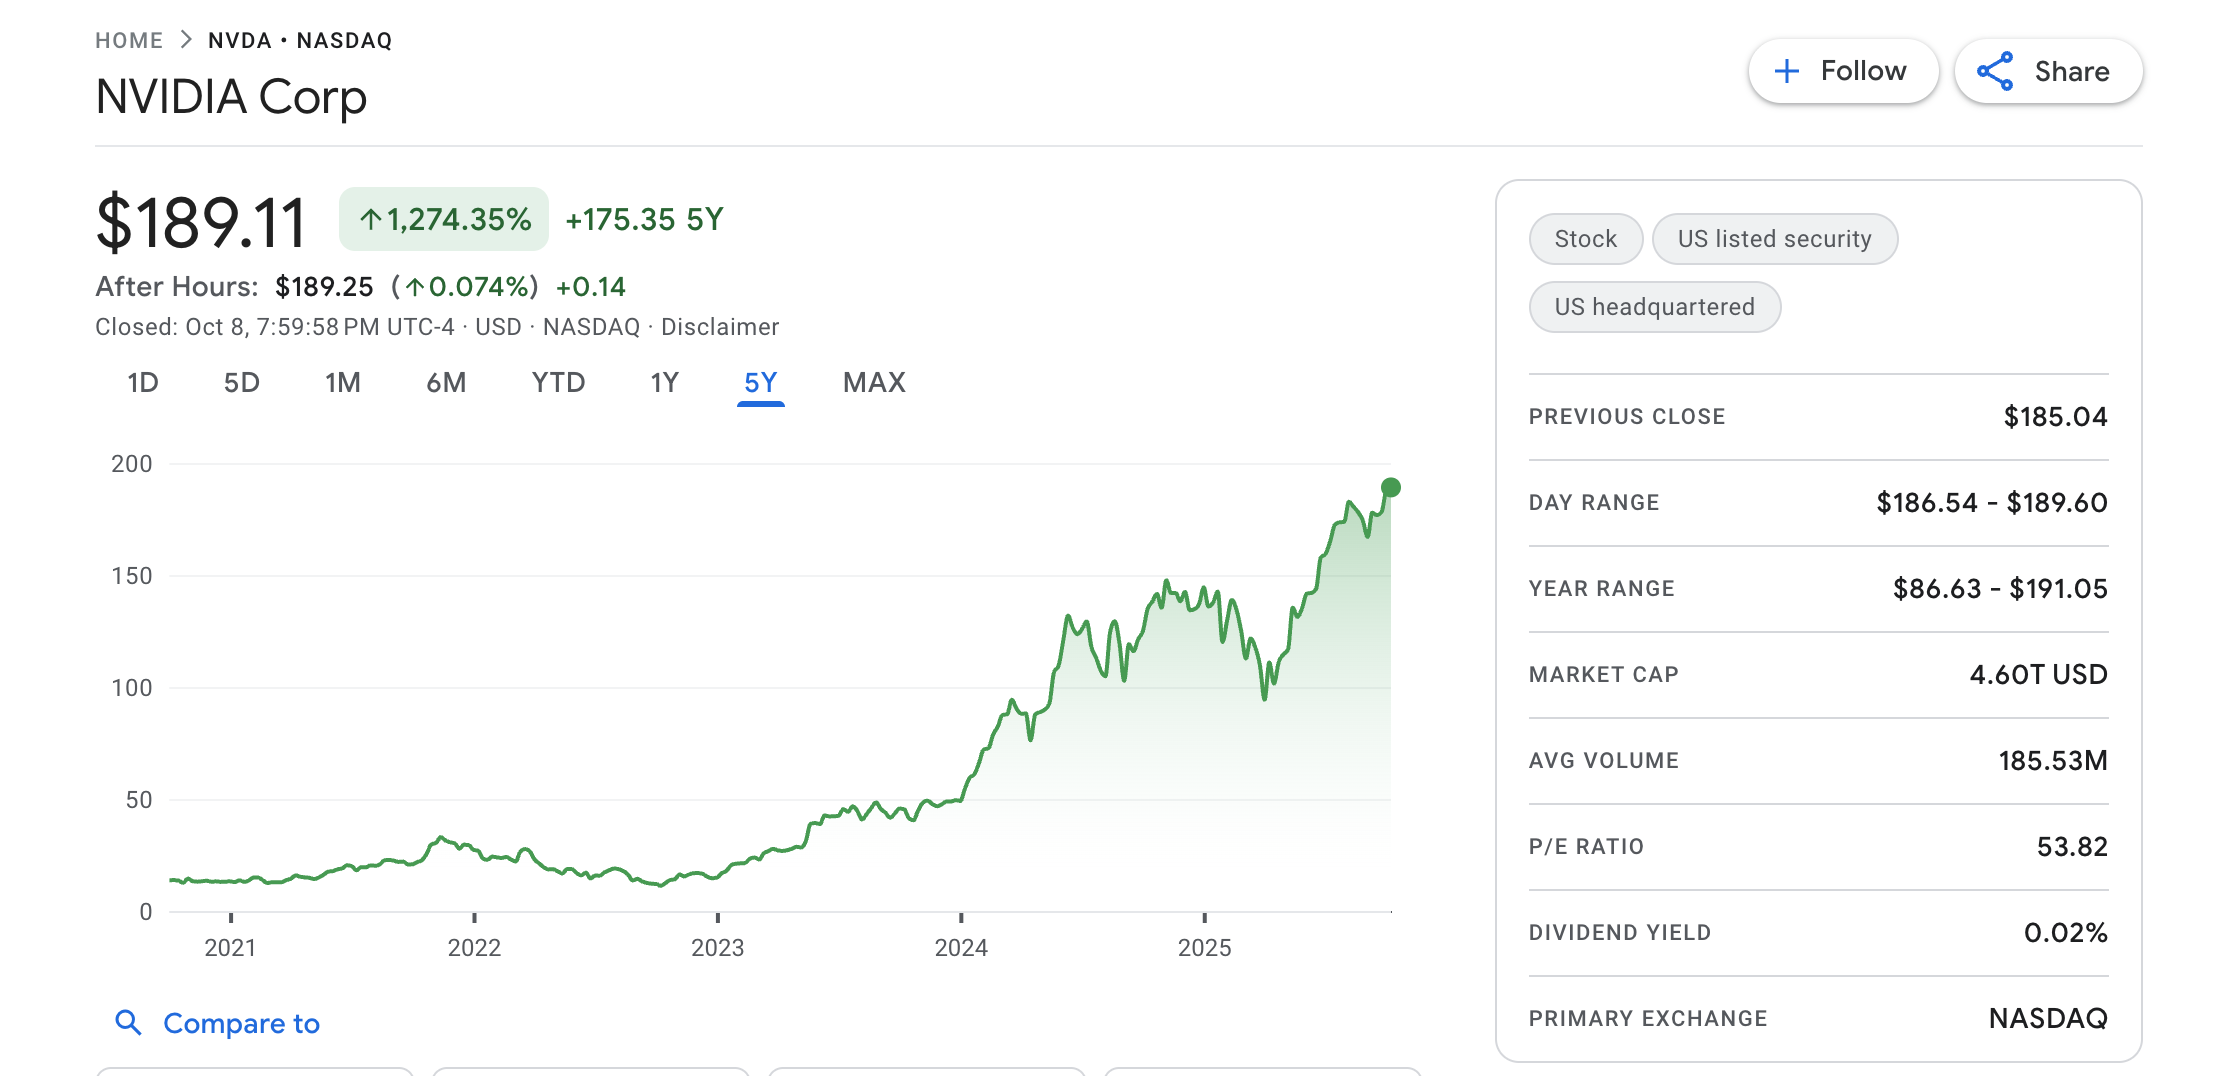
\includegraphics[width=1.0\textwidth,height=1.2\textheight,keepaspectratio]{images/nvidia_stock.png}
  \end{center}
\end{frame}

% Slide 2: Opening Question
\begin{frame}{GPUs are Everywhere Now}
  \begin{itemize}
    \item ChatGPT uses \textbf{over 30,000 NVIDIA GPUs} to handle \textbf{2.5+ billion queries daily}
    \item Each ChatGPT prompt uses 0.34 watt-hours of electricity
    \item Self-driving cars use GPUs for real-time processing
    \item Gaming has always used GPUs (the "G" is for Graphics!)
  \end{itemize}
  
  \vspace{1em}
  \Large \textbf{But why?}
\end{frame}

% Slide 2: A Relatable Problem
\begin{frame}{A Relatable Problem}
  \textbf{Question:} How long will it take me to reach Andheri?
  
  \vspace{1em}
  \begin{center}
    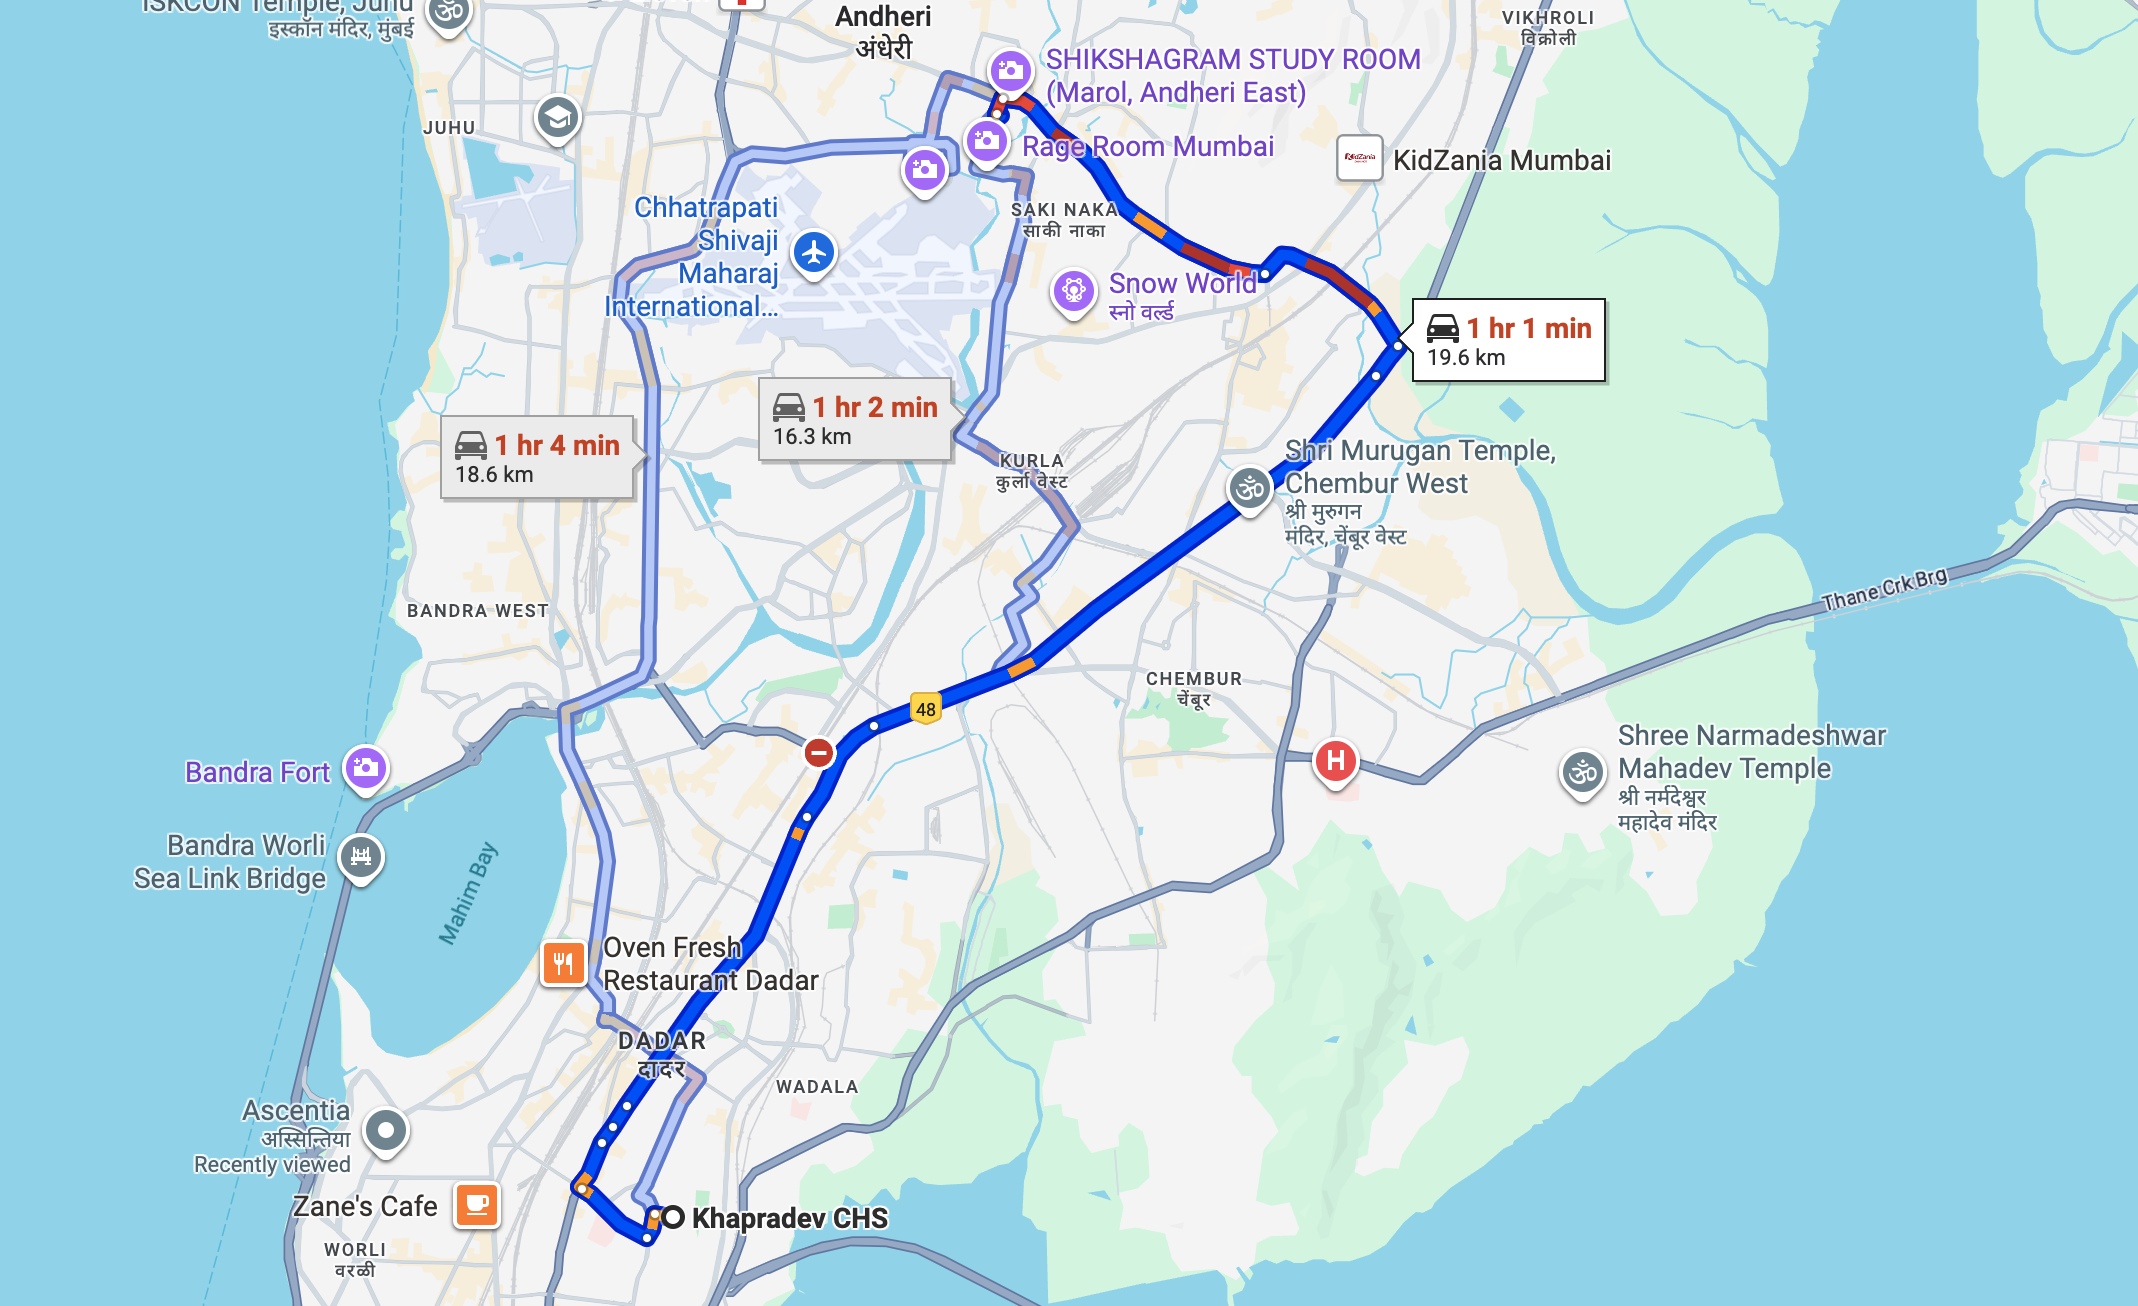
\includegraphics[width=0.7\textwidth,height=0.6\textheight,keepaspectratio]{images/mumbai_map.png}
  \end{center}
\end{frame}

% Slide 3: Features We Consider
\begin{frame}{What Affects Travel Time?}
  \begin{center}
    \vspace{2em}
    \Large
    \begin{itemize}
      \item Distance
      \item Time of day
      \item Is it raining?
      \item Weekday/Weekend
      \item Traffic conditions
    \end{itemize}
  \end{center}
\end{frame}

% Slide 4: Traditional vs ML Approach
\begin{frame}[fragile]{Two Approaches}
  \begin{block}{Traditional: Rule-Based}
    \small
    \begin{itemize}
      \item IF distance $>$ 15km THEN add 20 min
      \item IF is\_raining AND traffic $>$ 50\% THEN multiply by 1.5
      \item IF is\_weekend THEN subtract 10 min
      \item IF time\_of\_day between 8-10am OR 5-8pm THEN add 25 min
      \item IF construction\_zones $>$ 0 THEN add 5 min per zone
      \item ... (hundreds of nested rules!)
    \end{itemize}
  \end{block}
  
  \vspace{0.5em}
  
  \begin{block}{Machine Learning}
    Convert everything to numbers, learn a function from data
  \end{block}
  
  \vspace{0.5em}
  \small We won't cover the learning part today, just the prediction part!
\end{frame}

% Slide 5: Simple Prediction Formula
\begin{frame}{Making a Prediction}
  For one location, we do:
  
  \vspace{0.5em}
  \begin{align*}
    \text{predicted\_time} = &\; \text{distance} \times w_1 \\
    &+ \text{time\_of\_day} \times w_2 \\
    &+ \text{is\_raining} \times w_3 \\
    &+ \text{is\_weekend} \times w_4
  \end{align*}
  
  \vspace{0.5em}
  \begin{itemize}
    \item \textbf{Features}: distance, time\_of\_day, etc. (your input data)
    \item \textbf{Weights} ($w_1, w_2, w_3, w_4$): learned from data
    \item Weights are also called \textbf{model parameters}
  \end{itemize}
\end{frame}

% Slide 6: Scaling Up
\begin{frame}{But What If...}
  \begin{itemize}
    \item We have \textbf{1000 features} instead of 4?
    \item We want to predict for \textbf{10,000 locations} at once?
    \item We have \textbf{multiple layers} of transformations? (deep learning)
  \end{itemize}
  
  \vspace{2em}
  \centering
  \Large This becomes \textbf{matrix multiplication}
\end{frame}

% Slide 7: Matrix Multiplication
\begin{frame}{Matrix Multiplication}
  % TODO: Add image showing matrix multiplication with actual distance/time data
  % showing 10 locations x 5 features multiplied by 5 weights to get 10 predictions
  \begin{center}
    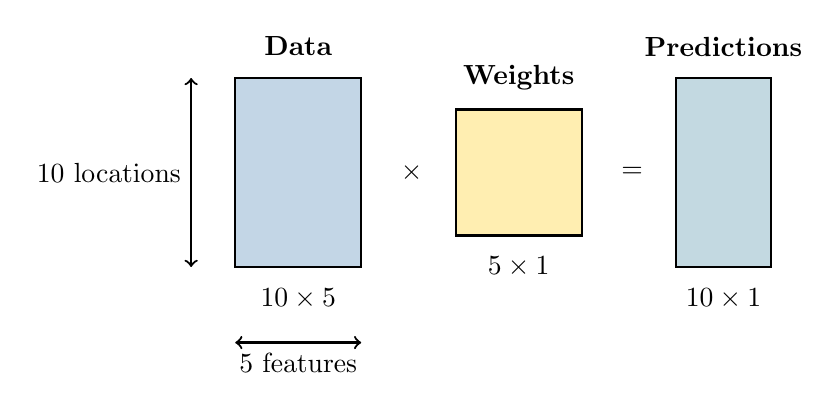
\begin{tikzpicture}[scale=0.8]
      % Matrix A (Data: locations x features)
      \draw[fill=pythonblue!30, thick] (0,0) rectangle (2,3);
      \node at (1, 3.5) {\textbf{Data}};
      \node at (1, -0.5) {$10 \times 5$};
      
      % Multiplication sign
      \node at (2.8, 1.5) {$\times$};
      
      % Matrix B (Weights)
      \draw[fill=pythonyellow!40, thick] (3.5,0.5) rectangle (5.5,2.5);
      \node at (4.5, 3) {\textbf{Weights}};
      \node at (4.5, 0) {$5 \times 1$};
      
      % Equals sign
      \node at (6.3, 1.5) {$=$};
      
      % Result Matrix C (Predictions)
      \draw[fill=pythonlightblue!40, thick] (7,0) rectangle (8.5,3);
      \node at (7.75, 3.5) {\textbf{Predictions}};
      \node at (7.75, -0.5) {$10 \times 1$};
      
      % Annotations
      \draw[<->, thick] (0,-1.2) -- (2,-1.2) node[midway, below] {5 features};
      \draw[<->, thick] (-0.7,0) -- (-0.7,3) node[midway, left] {10 locations};
    \end{tikzpicture}
  \end{center}
  
  \vspace{0.5em}
  \small Interactive demo: \texttt{http://matrixmultiplication.xyz/}
\end{frame}

% Slide 8: The Scale
\begin{frame}{The Real Scale}
  \textbf{Modern ML models:}
  
  \vspace{1em}
  \begin{itemize}
    \item GPT-3: 175 \textbf{billion} parameters
    \item Billions of multiply-add operations per prediction
    \item Training involves trillions of operations
  \end{itemize}
  
  \vspace{2em}
  \centering
  \Large How do we compute this efficiently?
\end{frame}

% Slide 9: Matrix Multiplication Characteristics
\begin{frame}{Why Matrix Multiplication is Special}
  \textbf{Perfect for parallel computing:}
  
  \vspace{1em}
  \begin{enumerate}
    \item \textbf{Embarrassingly Parallel}
    \begin{itemize}
      \item Each element can be computed independently
      \item No coordination needed between computations
    \end{itemize}
    
    \vspace{0.5em}
    \item \textbf{Simple Operations}
    \begin{itemize}
      \item Just multiply and add: $a \times b + c \times d + ...$
      \item Same operation repeated millions of times
    \end{itemize}
    
  \end{enumerate}
\end{frame}

% Slide 10: CPU Architecture
\begin{frame}{CPU: The Generalist}
  \begin{columns}[T]
    \begin{column}{0.5\textwidth}
      \textbf{Few powerful cores}
      \begin{itemize}
        \item 4-16 cores typically
        \item Sequential processing
        \item Great for general tasks
        \item \textbf{Latency-oriented design}
      \end{itemize}
      
      \vspace{1em}
      \textbf{Analogy:} 8 very smart people solving 10,000 problems one by one
    \end{column}
    \begin{column}{0.5\textwidth}
      \begin{center}
        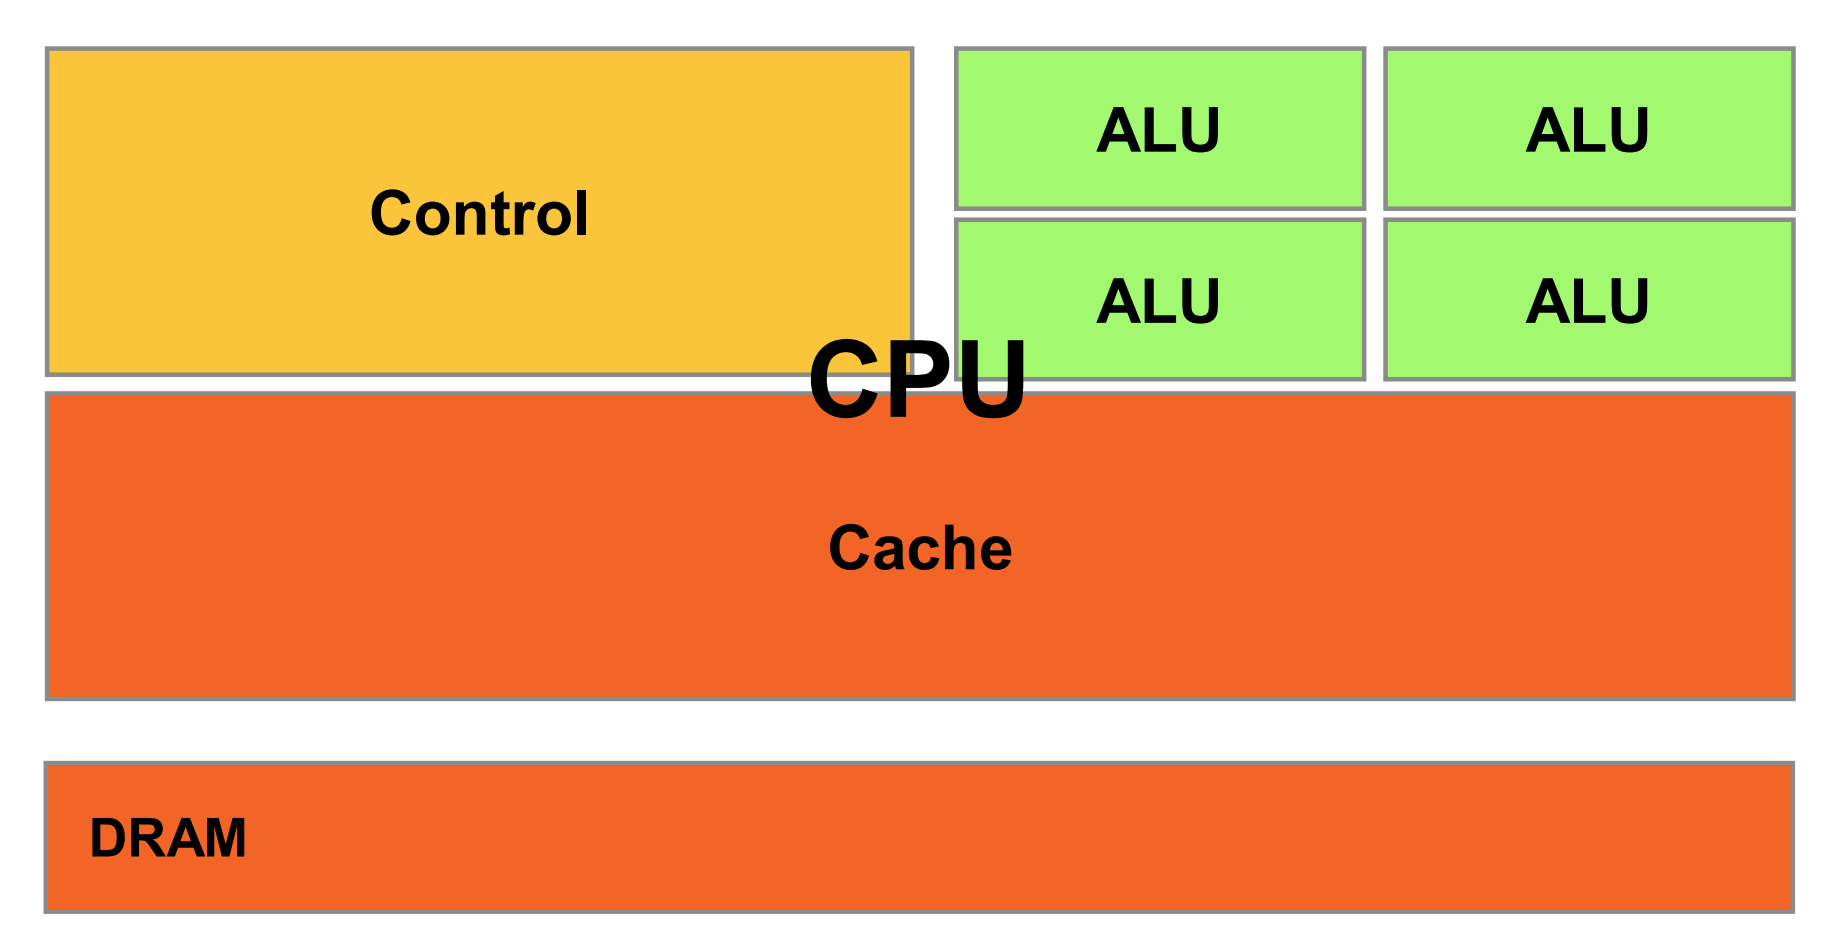
\includegraphics[width=\textwidth,height=0.6\textheight,keepaspectratio]{images/cpu_arch.png}
      \end{center}
    \end{column}
  \end{columns}
\end{frame}

% Slide 10: GPU Architecture
\begin{frame}{GPU: The Parallel Powerhouse}
  \begin{columns}[T]
    \begin{column}{0.5\textwidth}
      \textbf{Thousands of smaller cores}
      \begin{itemize}
        \item 10,000+ CUDA cores
        \item Parallel processing
        \item Specialized for repetitive tasks
        \item \textbf{Throughput-oriented design}
      \end{itemize}
      
      \vspace{1em}
      \textbf{Analogy:} 10,000 people each solving one problem simultaneously
    \end{column}
    \begin{column}{0.5\textwidth}
      \begin{center}
        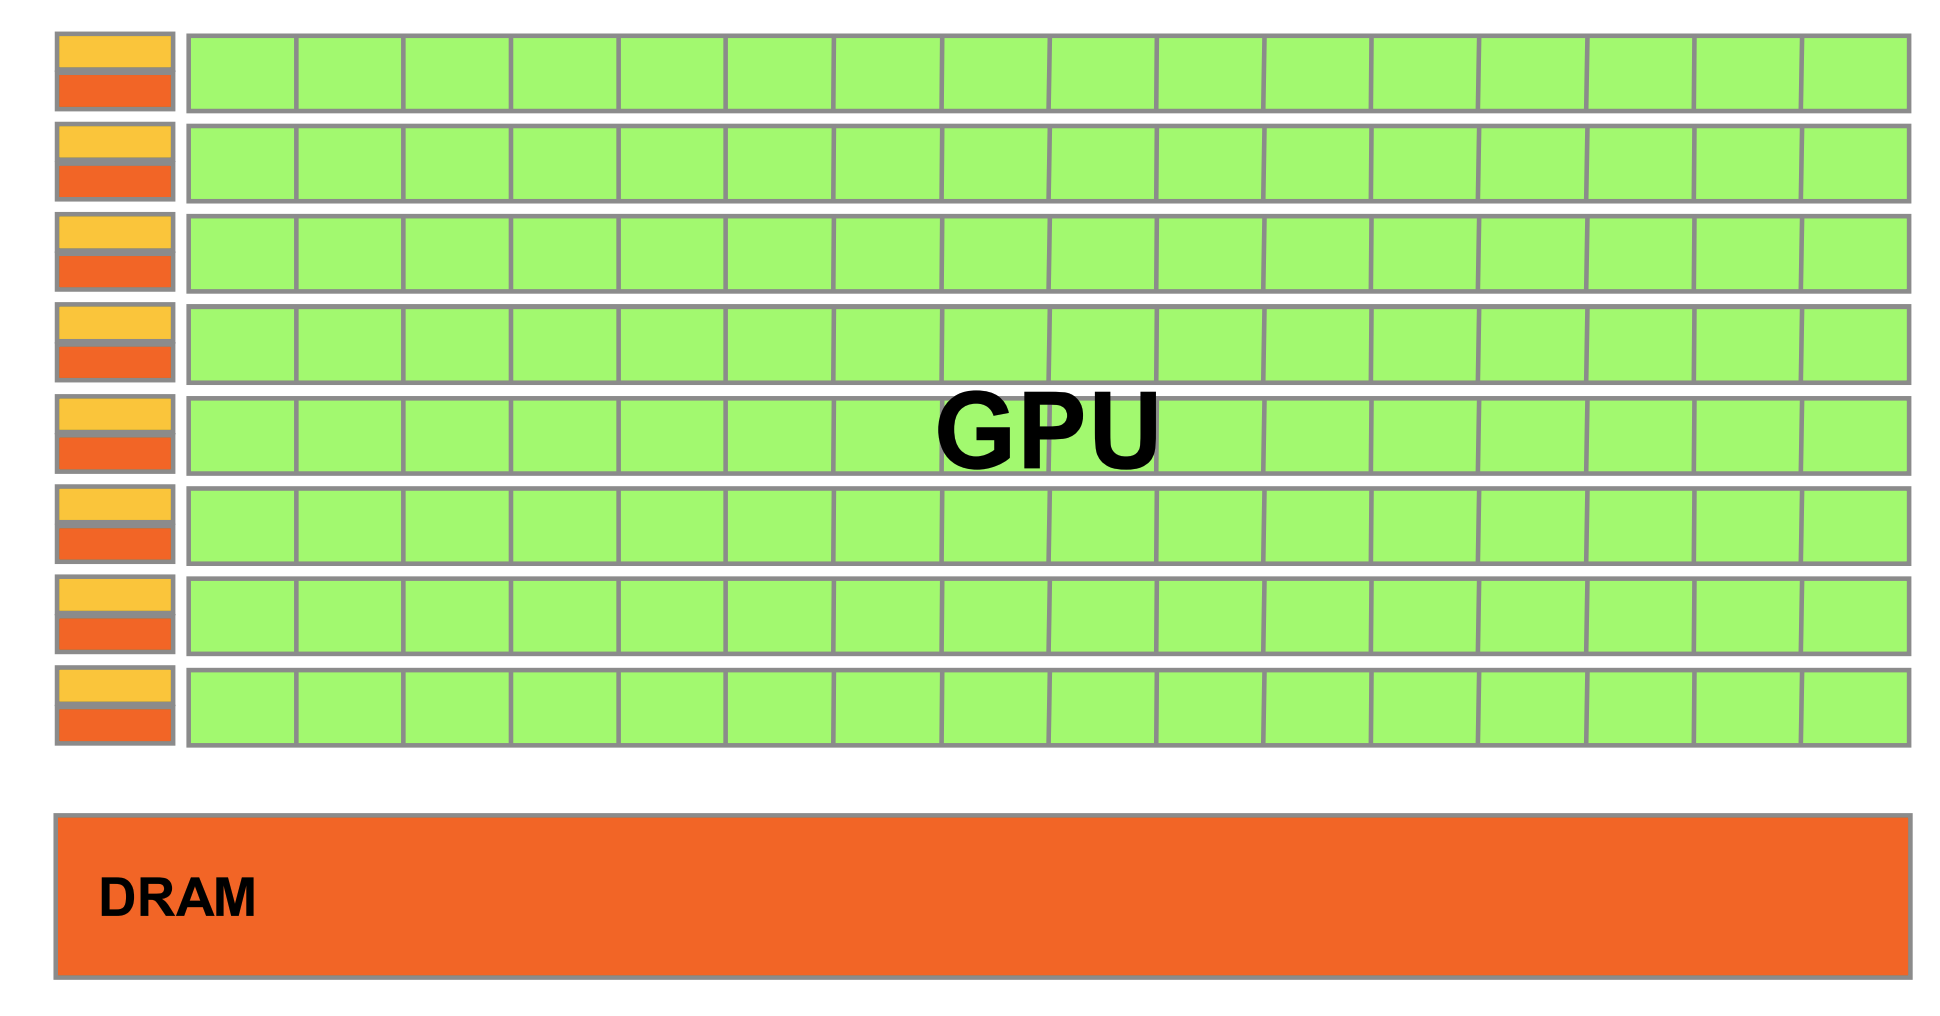
\includegraphics[width=\textwidth,height=0.6\textheight,keepaspectratio]{images/gpu_arch.png}
      \end{center}
    \end{column}
  \end{columns}
\end{frame}

% Slide 11: Matrix Operations for Graphics
\begin{frame}{Matrix Operations in Graphics}
  \textbf{How matrices rotate and move objects in 3D space:}
  
  \vspace{0.5em}
  \begin{center}
    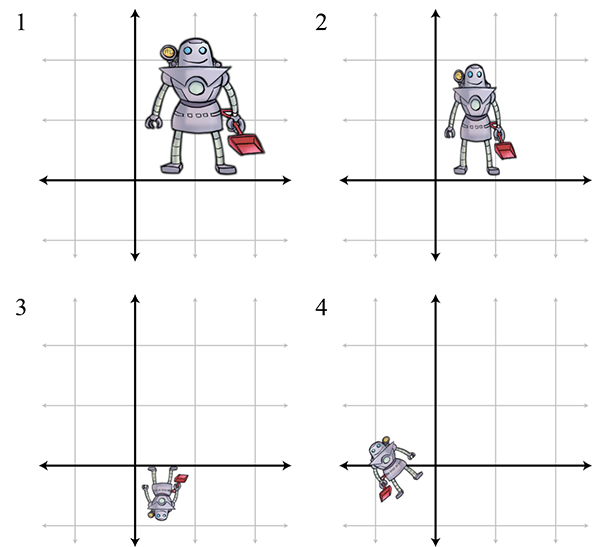
\includegraphics[width=0.85\textwidth,height=0.7\textheight,keepaspectratio]{images/exercise_match_matrix_to_picture.png}
  \end{center}
\end{frame}

% Slide 12: Why GPUs Originally
\begin{frame}{Why GPUs Exist}
  GPUs were originally designed for \textbf{graphics and gaming}
  
  \vspace{1em}
  \begin{itemize}
    \item 3D transformations: matrix operations
    \item Rendering millions of pixels: parallel
    \item Real-time requirements: fast
  \end{itemize}
  
  \vspace{1em}
  \centering
  \textbf{Turns out:} AI has the same needs!
\end{frame}

% Slide 14: Demo Section Title
\begin{frame}[standout]
  \Huge Seeing is Believing
  
  \vspace{1em}
  \Large Python Timing Examples
\end{frame}

% Slide 15: Demo 1 Setup
\begin{frame}[fragile]{Demo 1: NumPy vs CuPy}
  \textbf{Setup:} Large matrix multiplication (5000 × 5000)
  
  \vspace{0.5em}
  \begin{columns}[T]
    \begin{column}{0.48\textwidth}
      \textbf{CPU (NumPy)}
      \tiny
\begin{verbatim}
import numpy as np
import time

size = 5000
A = np.random.rand(size, size)
B = np.random.rand(size, size)

start = time.time()
C = A @ B
end = time.time()

print(f"Time: {end-start:.3f}s")
# Result: 1.026s
\end{verbatim}
    \end{column}
    \begin{column}{0.48\textwidth}
      \textbf{GPU (CuPy)}
      \tiny
\begin{verbatim}
import cupy as cp
import time

size = 5000
A = cp.random.rand(size, size)
B = cp.random.rand(size, size)

start = time.time()
C = A @ B
cp.cuda.Stream.null.synchronize()
end = time.time()

print(f"Time: {end-start:.3f}s")
# Typical result: ~0.015s
\end{verbatim}
    \end{column}
  \end{columns}
\end{frame}

% Slide 16: Demo 1 Results
\begin{frame}{Demo 1: Results}
  \textbf{Matrix Multiplication: 5000 × 5000}
  
  \vspace{1em}
  \begin{center}
    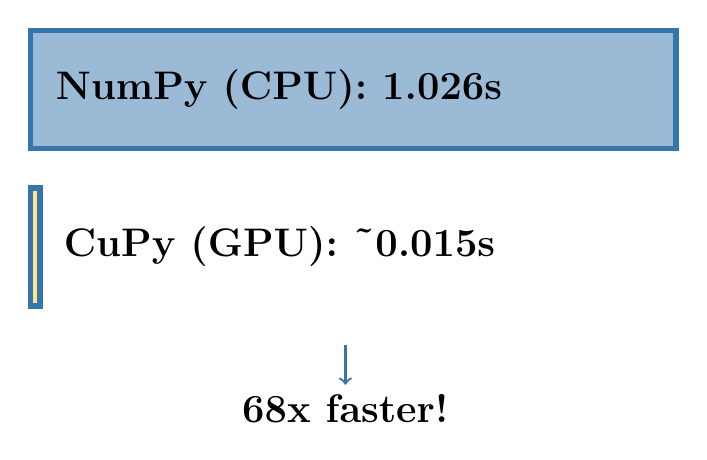
\begin{tikzpicture}
      % CPU bar
      \draw[fill=pythonblue!50, draw=pythonblue, line width=2pt] (0,0) rectangle (8.2,1.5);
      \node[right] at (0.2,0.75) {\Large\textbf{NumPy (CPU): 1.026s}};
      
      % GPU bar
      \draw[fill=pythonyellow!60, draw=pythonblue, line width=2pt] (0,-2) rectangle (0.12,-0.5);
      \node[right] at (0.3,-1.25) {\Large\textbf{CuPy (GPU): \textasciitilde0.015s}};
      
      % Speedup annotation
      \draw[->, thick, pythonblue] (4,-2.5) -- (4,-3);
      \node[below] at (4,-3) {\Large\textbf{68x faster!}};
    \end{tikzpicture}
  \end{center}
  
  \vspace{1em}
  \small \textit{NumPy result measured on this system. GPU time is typical for NVIDIA RTX GPUs.}
\end{frame}


% Slide 19: When Should You Care?
\begin{frame}{When Should You Care About GPUs?}
  \textbf{Use GPUs when you have:}
  
  \vspace{1em}
  \begin{itemize}
    \item Large matrices (thousands of rows/columns)
    \item Repeated operations (training loops)
    \item Real-time requirements
    \item Deep learning models
  \end{itemize}
  
  \vspace{1em}
  \textbf{Skip GPUs for:}
  \begin{itemize}
    \item Small data (< 1000 elements)
    \item One-off calculations
    \item Overhead of data transfer > computation time
  \end{itemize}
\end{frame}

% Slide 20: How to Get Started
\begin{frame}{How to Get Started}
  \textbf{Free options:}
  \begin{itemize}
    \item \textbf{Google Colab} - Free T4 GPU access
    \item \textbf{Kaggle Notebooks} - Free GPU hours
  \end{itemize}
  
  \vspace{1em}
  \textbf{Cloud providers:}
  \begin{itemize}
    \item AWS, Google Cloud, Azure
    \item Pay per hour of GPU usage
  \end{itemize}
  
  \vspace{1em}
  \textbf{Local GPU:}
  \begin{itemize}
    \item NVIDIA GPUs (required for CUDA)
    \item For serious/regular ML work
  \end{itemize}
\end{frame}

% Slide 21: Python Tools
\begin{frame}{Python Tools for GPU Computing}
  \begin{description}
    \item[PyTorch] Most popular for deep learning, easy GPU support
    \item[TensorFlow] Google's framework, mature ecosystem
    \item[CuPy] NumPy, but on GPU
    \item[JAX] Google's new framework, automatic differentiation
    \item[RAPIDS] GPU-accelerated data science (pandas-like)
  \end{description}
  
  \vspace{1em}
  \centering
  \small Most just need \texttt{.to('cuda')} or similar!
\end{frame}

% Slide 22: Summary
\begin{frame}{Putting It All Together}
  \begin{enumerate}
    \item Modern AI = \textbf{lots of matrix multiplication}
    \item Matrix multiplication = \textbf{embarrassingly parallel}
    \item CPUs = sequential, GPUs = \textbf{parallel powerhouses}
    \item Result: \textbf{50-200x speedup} for ML workloads
  \end{enumerate}
  
  \vspace{2em}
  \centering
  \Large That's why every AI breakthrough mentions "GPU hours"!
\end{frame}

% Slide 23: Thank You
\begin{frame}[standout]
  \Huge Thank You!
  
  \vspace{2em}
  \Large Questions?
\end{frame}

\end{document}

